\documentclass[sigplan,screen]{acmart}
\AtBeginDocument{%
  \providecommand\BibTeX{{%
    \normalfont B\kern-0.5em{\scshape i\kern-0.25em b}\kern-0.8em\TeX}}}

\begin{document}

\title{Comparative Study of Memory Allocators}

\author{Arun Kumar}
\affiliation{%
  \institution{114708780}}

\author{Namrata Balwani}
\affiliation{%
  \institution{115192977}}

\author{Prajjawal Agarwal}
\affiliation{%
 \institution{115134849}}


%% ======= ABSTRACT =======.
\begin{abstract}
  Memory allocation is a critical component of system performance and resource management. With the increasing usage of memory by high-workload applications, there is a need for efficient memory allocation by the operating systems in order to improve program performance and reduce memory usage.

    In this paper, we evaluate the performance of several popular memory allocators, on some benchmarks. We measure the performance of each allocator in terms of memory usage, fragmentation, and latency, and compare the results across different benchmarks and configurations. In addition, we use hardware performance monitoring tools such as valgrind and Linux perf to gather statistics on cache misses and memory heaps and use flame graphs to visualize the results. Our findings show that the choice of memory allocator can have a significant impact on system performance and that certain allocators may be better suited for specific workloads.
\end{abstract}

\ccsdesc[500]{Memory Management~Performance Analysis}
\ccsdesc[300]{Memory Management~Debugging and profiling}
\ccsdesc{Memory Management~Empiricial Studies}

\keywords{dynamic memory allocators, benchmarks,\\ 
linux perf tool, valgrind, memcheck, massif, flamegraphs}


\maketitle

%% ======= INTRODUCTION =======.

\section{Introduction}
In order to successfully assign memory to running processes, an operating system must effectively manage the system's available memory. Efficient memory allocation can help prevent memory shortages, which can cause programs to crash or the operating system to become unstable. Dynamic memory allocators are used to allocate memory dynamically during the execution of a program, as opposed to allocating memory statically at compile-time. 

There are several dynamic memory allocators currently available, each of which was made for different use cases such as CPU-intensive, memory-intensive, and multithreaded applications. There have been few works done in this area to compare different memory allocators for different benchmark applications \cite{berger2001composing}. Inspired by those works we have tried comparing some general-purpose memory allocators for a different set of benchmarks. We have used five different memory allocators which are described in the next sub-sections:

\subsection{jemalloc}
jemalloc is a general-purpose malloc(3) implementation that emphasizes fragmentation avoidance and scalable concurrency support.  It was first created as a FreeBSD-specific library, but it has now been ported to a variety of other systems and is freely accessible\cite{evans2006scalable}.

\subsection{SuperMalloc}
SuperMalloc is an implementation of malloc(3) originally designed for X86 Hardware Transactional Memory (HTM)\cite{kuszmaul2015supermalloc}. This is a highly scalable allocator beneficial for parallel programs running on multicore processors. SuperMalloc's capacity to manage several threads without experiencing significant contention or lock overhead is one of its main benefits.

\subsection{ptmalloc}
ptmalloc is the standard memory allocator used in libc library. It aims to minimize cache misses by grouping together small objects that are likely to be allocated together. When compared to other memory allocators, one of the important characteristics of ptmalloc is its capacity to decrease lock contention in multi-threaded applications.

\subsection{Hoard}
Hoard is a Scalable Memory Allocator for Multithreaded Applications primarily focussing on improving performance through speed, scalability, false sharing avoidance, and low fragmentation \cite{berger2000hoard} It's capacity to manage numerous threads without experiencing severe lock contention or synchronization costs is one of its main advantages.

\subsection{TCMalloc}
TCMalloc is Google's customized implementation of C's malloc() and C++'s operator newly used for memory allocation within our C and C++ code. It is a fast, multi-threaded malloc implementation and is made to handle numerous threads concurrently without slowing down.


\section{Methodologies}
In this paper, we are trying to evaluate the performance of various popularly used dynamic memory allocation algorithms such as jemalloc, SuperMalloc, hoard, TCMalloc, and ptmalloc. We use six dynamic memory management intensive benchmarks from various sources to evaluate the memory allocators. 

We have chosen benchmarks that are essentially allocation-intensive and have a large amount of live data for which space cost will matter the most and hence will enable us to differentiate between the various allocator’s performances. In addition, some of our measurements of memory usage may introduce errors of up to 4 or 5 KB in bad cases; we wanted to ensure that these errors were generally small relative to the actual memory usage and fragmentation. 

We tried to obtain a variety of traces, including several that are widely used as well as CPU and memory-intensive\cite{johnstone1998memory}. We also tried to evaluate the performance on the basis of single and multithreaded applications to get an insight into how the allocators perform when there is a careful consideration of parallel processing, concurrent accesses, and scalability in general for the multithreaded environment versus the single-threaded one. 

The next subsections contain the benchmarks that were used and the details about our experimental study.

\subsection{Single threaded benchmarks}

\subsubsection{espresso}
espresso is a widely used optimizer for programmable logic arrays, described by Grunwald, Zorn, and Henderson\cite{grunwald1993improving}. The benchmark is used in the context of cache-aware memory allocation.

\subsubsection{cfrac}
cfrac by Dave Barrett, is an implementation to factor large integers using the continued fraction factorization method. The original application uses explicit reference counting to reclaim storage\cite{gay1998memory}.

\subsubsection{gs}
Ghostscript is a widely-used portable interpreter for PostScript\cite{johnstone1998memory} and PDF files. We used a benchmark that makes Ghostscript process the entire Intel Software Developer’s Manual PDF, which is around 5000 pages.

\subsubsection{lua}
Lua is a lightweight scripting language that is often used for embedded systems and other resource-constrained environments. The benchmark compiles the lua interpreter with the goal to measure the allocator's performance in terms of speed and memory usage.

\subsubsection{redis}
We are running redis-benchmark, with 1 million requests pushing 10 new list elements and then requesting the head 10 elements, and measuring the requests handled per second. This benchmark simulates a real-world workload.

\subsection{Multi threaded benchmarks}

\subsubsection{Larson}
Larson simulates a server workload using 100 separate threads which each allocate and free many objects but leaves some objects to be freed by other threads. Also, it uses sized deallocation calls which have a fast path in some allocators \cite{larson1998memory}. This benchmark is used to evaluate memory allocation metrics for long-running  server  applications and scalability on SMP systems.

\subsection{Experimental study}

In this experimental study, we used the Mimalloc-bench, an open-source suite for benchmarking malloc implementations \cite{mimallocGit}, which is a collection of various benchmarks from the academic literature and memory allocators. We wrote various scripts to run hardware monitoring tools such as Linux perf to collect CPU data during the execution for a given set of benchmarks and memory allocators and visualized this data using flame graphs to validate our observations. Additionally, we modified a few scripts in the test suite for fetching the data from the Valgrind tool to get the memory allocation and fragmentation details for each allocator on various benchmarks. This data was then converted into normalized graphical representations using some additional scripts.

\section{Experimental Setup}
An x86\textunderscore64-architectured computer system that could run in both 32-bit and 64-bit CPU op-modes was used. The machine had 16GB of RAM and a dual-core CPU that could handle two threads running in parallel on each core. A 2.80GHz Intel(R) Xeon(R) Platinum 8370C CPU was chosen as the specific CPU model. Through the VT-x technology, the system also included virtualization capabilities, with Microsoft serving as the hypervisor vendor. The type of virtualization employed was full.

\section{Result}
This investigation provides several insights when it comes to time and memory optimization. All the figures and results that we presented in this investigation are normalized on our standard ptmalloc allocator which is standard on most Linux machines.

We present a comparison of the runtimes of our benchmark applications normalized to the original sys or ptmalloc allocator. We have represented both sys (or the kernel) time and the total time taken by these benchmarks as shown in \figurename{ \ref{systime}} and \figurename{ \ref{tottime}} respectively. 

We can see that the average total time taken by all allocators is more or less similar for all benchmarks except we see hoard, SuperMalloc, and TCMalloc performing better on multithreading workloads like Larson. With the kernel runtime, we see that the SuperMalloc performs extremely well for the Larson benchmark with low page faults (see \figurename{ \ref{page_faults}}), almost showing 70\% better performance compared to the others, because it uses hardware transactional memory to speed up parallel operations which is useful in the multithreaded Larson application.

For the two extremely allocation-intensive benchmarks, cfrac and lua, we also observed that SuperMalloc performs worst on both cfrac and lua compared to other allocators, which we suspect is because SuperMalloc is optimized for low memory fragmentation and thus incurs additional overhead when from extra virtual memory allocations \cite{kuszmaul2015supermalloc}.

An interesting observation was that the number of bytes allocated (see \figurename{ \ref{memtable}}) was the same among jemalloc, hoard, SuperMalloc for benchmarks: cfrac, espresso, gs. For Larson benchmark number of bytes allocated vary for different allocators, ptmalloc assigns almost twice of jemalloc and SuperMalloc which has the least. We observed that for multi-threaded benchmarks, scalable allocators like hoard and SuperMalloc have performed better in almost all the metrics compared to our standard pt-malloc.

When it comes to external fragmentation (see \figurename{ \ref{ext_fragmentation}}), we observed SuperMalloc and hoard have fared better compared to all other allocators. Though we think our methodology to measure external fragments has some gap, it does account for padding present inside the allocated structure, and the general trend is the same as we expected to observe.

We use Redis to test whether the allocators can take on large numbers of requests and still maintain a high workload.  For almost all the allocators, we observed similar performances when it comes to time and external fragmentation. However, we observed significantly fewer page-faults for jemalloc and SuperMalloc nearly  15\% and 25\% compared to our standard allocator ptmalloc. 

We also built the flame graphs (see \figurename{ \ref{flame}}) using the perf tool and were able to correlate our results with the data presented there. But due to space constraints, a larger discussion cannot be done there.

We also calculated other metrics context switches, resident set size, no of free, and number of allocations. However, due to space constraints, we are not able to discuss everything, but both the normalized as well as the experimental data are available at our GitHub repo here \\ \href{https://github.com/prajjawal05/comparing-mallocs}{https://github.com/prajjawal05/comparing-mallocs}.


\begin{figure}
\centering
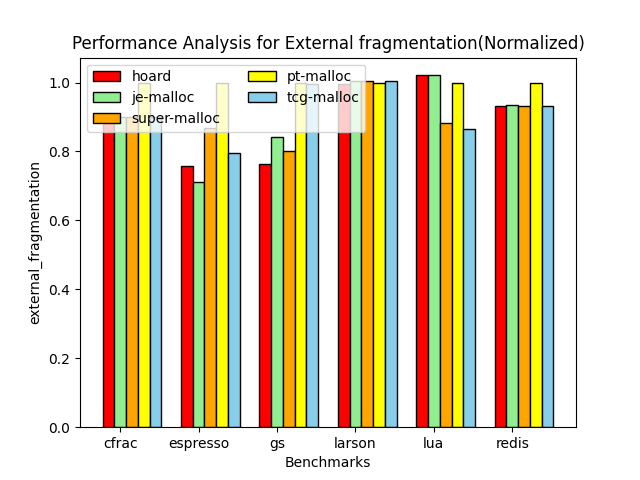
\includegraphics[width=0.4\textwidth, height=4.5cm]{External fragmentation(Normalized)_plot.png}
\caption{External fragmentation (Normalized)}
\label{ext_fragmentation}
\end{figure}

\begin{figure}
\centering
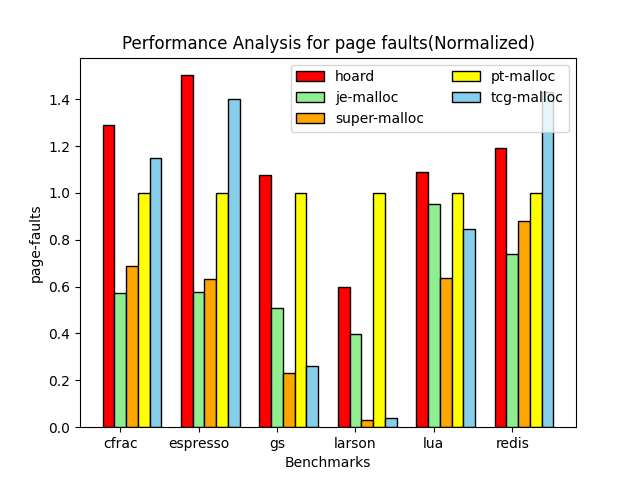
\includegraphics[width=0.40\textwidth, height=4.5cm]{page faults(Normalized)_plot.png}
\caption{Page Faults (Normalized)}
\label{page_faults}
\end{figure}

\begin{figure}
\centering
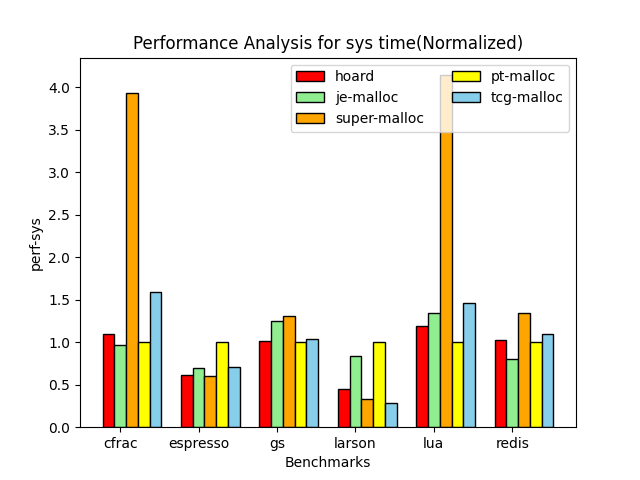
\includegraphics[width=0.4\textwidth, height=4.5cm]{sys time(Normalized)_plot.png}
\caption{Kernel run-time (Normalized)}
\label{systime}
\end{figure}

\begin{figure}
\centering
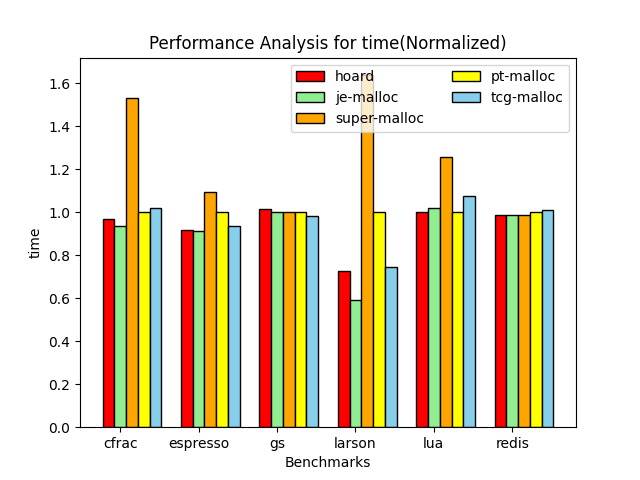
\includegraphics[width=0.4\textwidth, height=4.5cm]{time(Normalized)_plot.png}
\caption{Total time (Normalized)}
\label{tottime}
\end{figure}

\begin{figure}
\centering
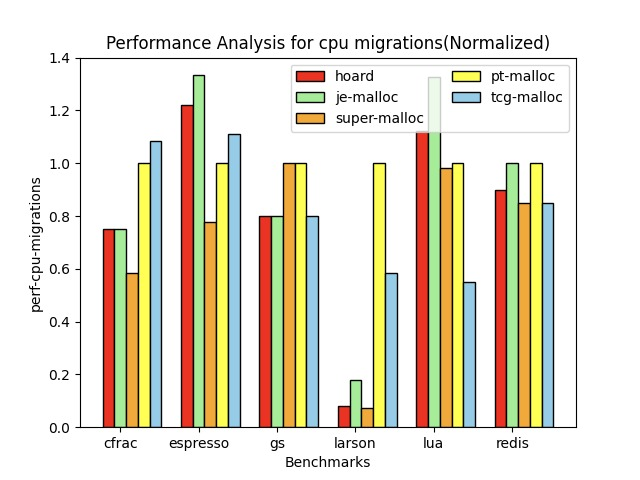
\includegraphics[width=0.4\textwidth, height=4.5cm]{cpu migrations.jpeg}
\caption{CPU Migrations (Normalized)}
\label{vue_snipp-4}
\end{figure}

% \begin{teaserfigure}
%   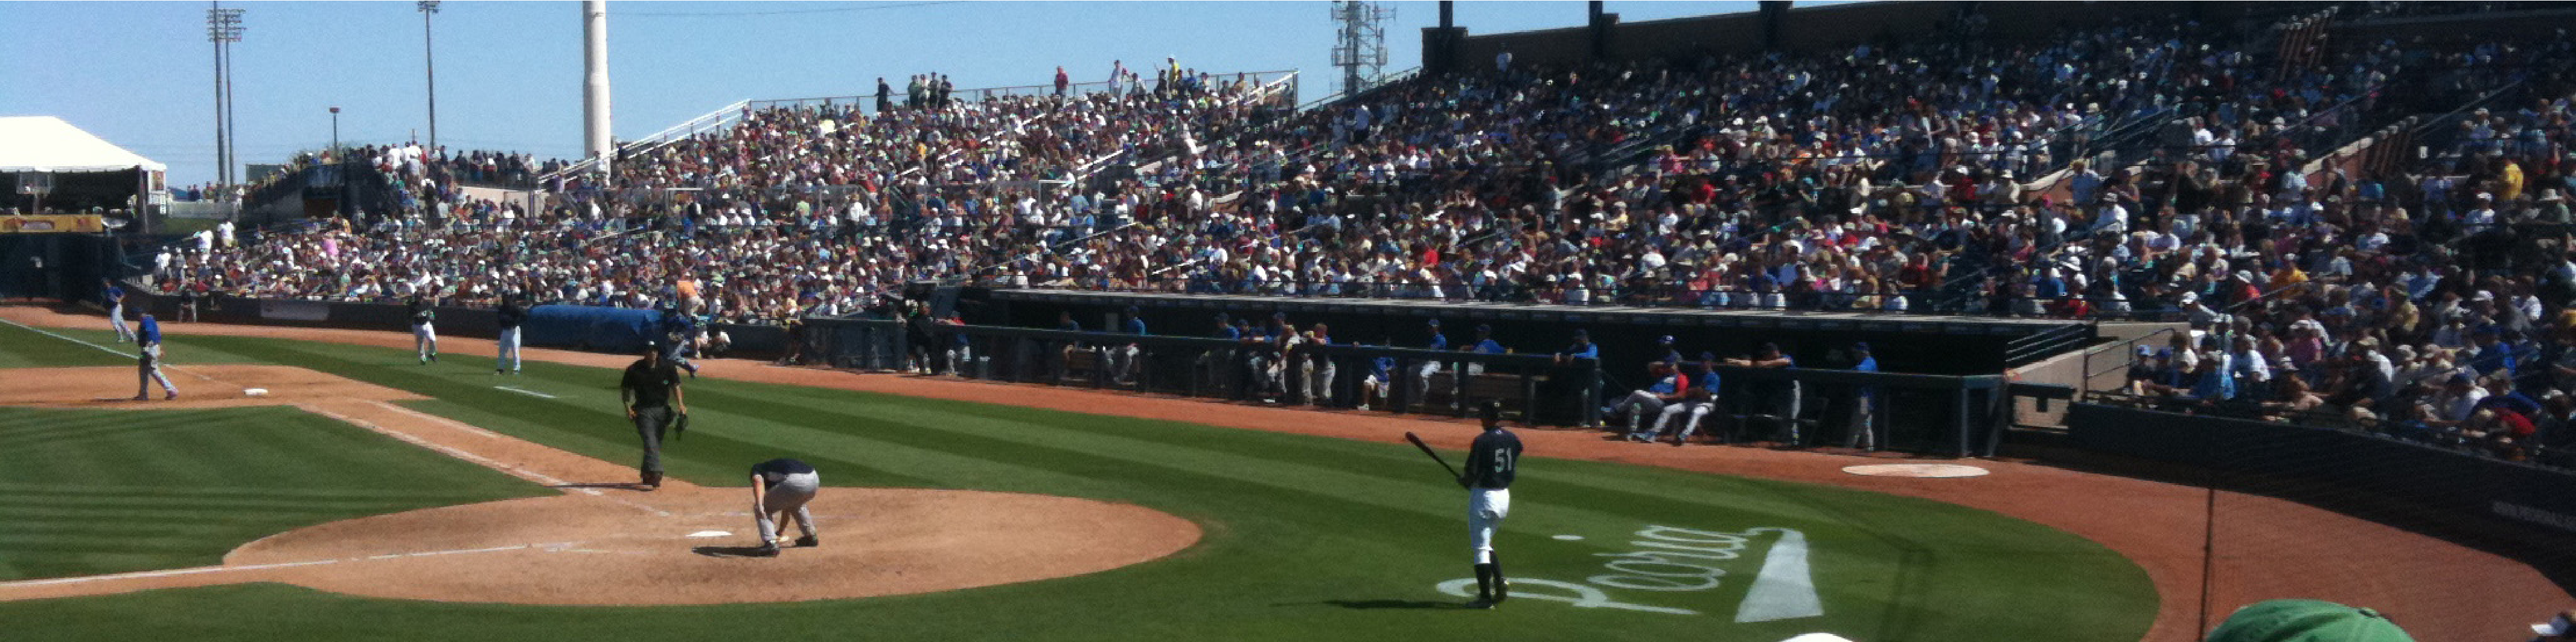
\includegraphics[width=\textwidth]{sampleteaser}
%   \caption{Seattle Mariners at Spring Training, 2010.}
%   \Description{Enjoying the baseball game from the third-base
%   seats. Ichiro Suzuki preparing to bat.}
%   \label{fig:teaser}
% \end{teaserfigure}


\begin{figure*}
\centering
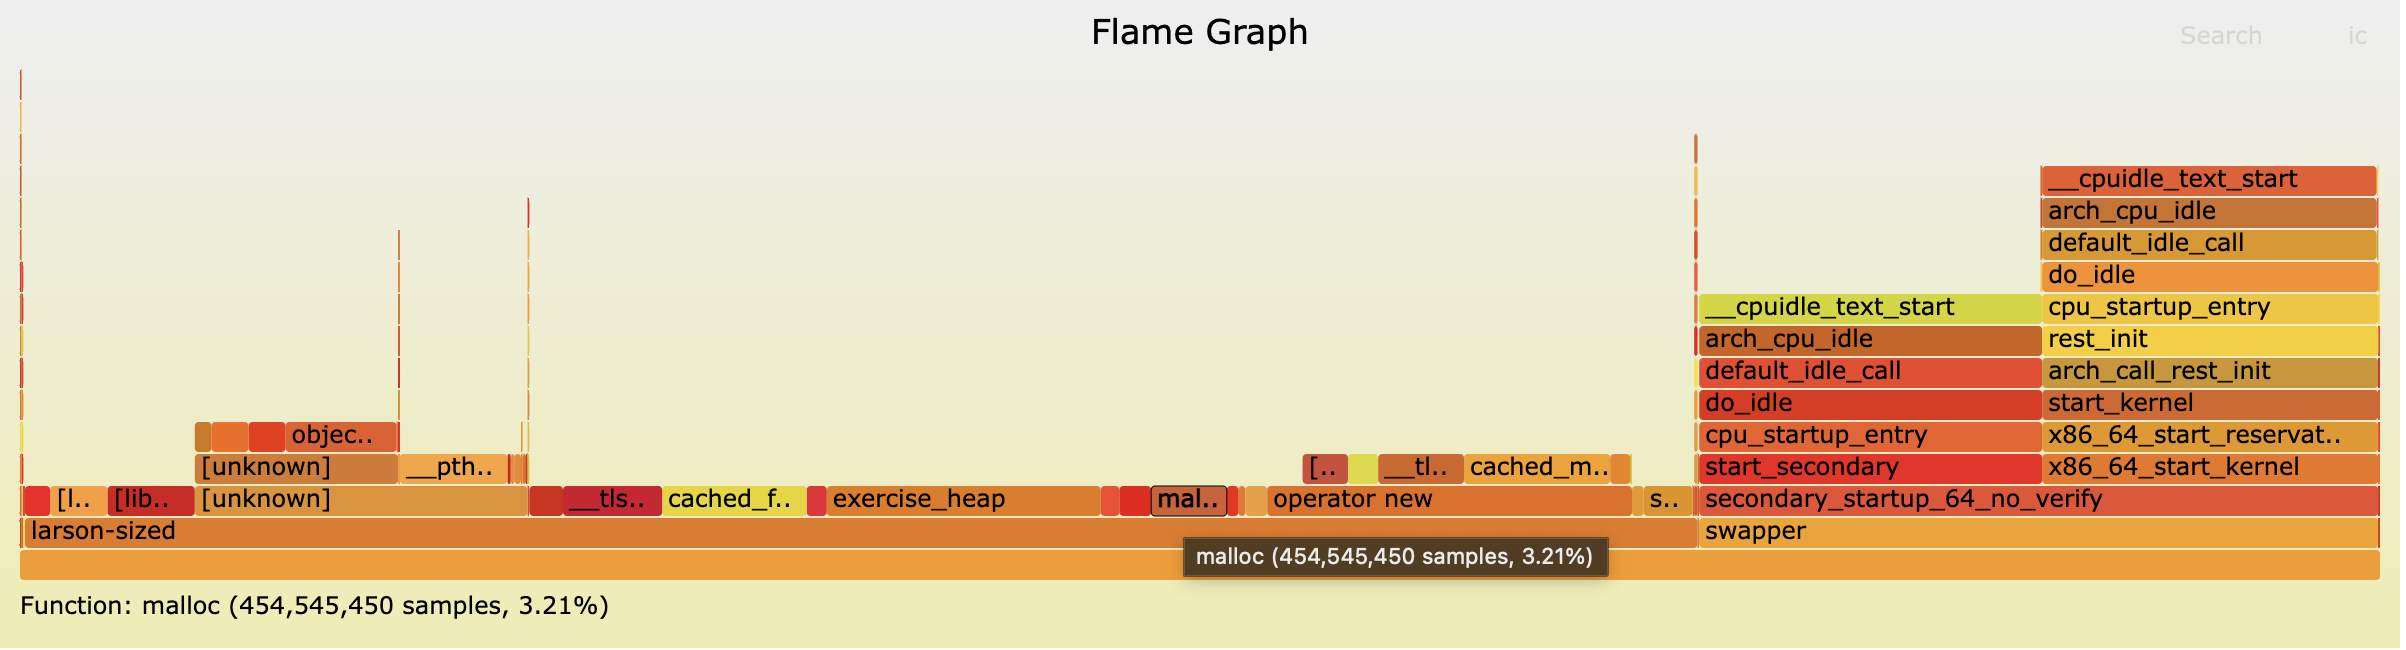
\includegraphics[width=0.95\textwidth, height=5.0cm]{flamegraph.png}
\caption{Flamegraph for Larson Benchmark with SuperMalloc}
\label{flame}
\end{figure*}

\begin{figure*}
\centering
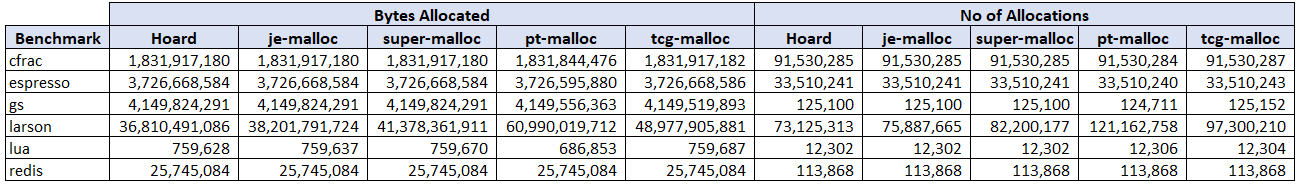
\includegraphics[width=0.95\textwidth, height=2.5cm]{table-memory.png}
\caption{Table showing the number of bytes allocated and the number of allocations for each benchmark application and a memory allocator.}
\label{memtable}
\end{figure*}

\section{Conclusions}
Dynamic memory management is a critical part of many important applications for which performance is crucial. Organizations like Facebook and Google,  in an effort to avoid the overhead of standard allocators like ptmalloc provided in Linux, often write their own custom allocation implementations in an effort to increase performance further. Our experiments with different benchmarks suggest allocators performed best when they are designed with the type of load they are expected to encounter.  Most of the allocator trade-offs include extra memory overhead or allocations and performance. Strategies like per thread  or processor allocations tend to provide performance benefits with extra memory overhead. Scalable allocators like Hoard and super malloc tend to perform better when they experience a multithreaded workload. 

During executing our experiments we encountered some issues. While trying to collect TLB misses data using Valgrind we faced some errors due to incompatible architectures. As we were running our test suite on a guest VM through a hypervisor, capturing this data was difficult and did not give appropriate results. There was a similar LLVM test suite which was officially provided by Microsoft, that we were not able to run because of the system compatibility issues with cmake tool. While running the Larson benchmark to collect data from Valgrind, it was taking a long time approx 9+ hrs to get the full data for 16 processes, we modified the script to capture the data without the memory leaks.

We believe our experimental results are explanatory, however, due to the high complexity in present applications it is difficult for us to pin-point the exact reasons for differences in performances. Future work should be directed more toward increasing the explainability of software performance and increasing the scope of performance metrics.

\section{Acknowledgement}
We would like to express our sincere gratitude to Professor Dongyoon Lee for his invaluable guidance and support throughout the duration of the project and course. His extensive knowledge and expertise in the field have been instrumental in shaping our understanding and helping us to achieve our goals.
  

\bibliographystyle{ACM-Reference-Format}
\bibliography{sample-base}

\end{document}
\endinput
%%
%% End of file `sample-sigplan.tex'.
